\subsubsection{Raspicontroller}
Der Raspicontroller ist für die Ablaufsteuerung und die Erkennung des Korbes zuständig. Die Applikation ist in Python geschrieben und wird als Service auf einem Raspberry Pi ausgeführt. Auf dem Raspberry Pi ist das Betriebssystem Arch Linux installiert. Arch Linux lässt sich ohne grafische Oberfläche betreiben, wodurch wenig Ressourcen verwendet werden. Das Betriebssystem lässt sich komplett über Textdateien konfigurieren. Der Raspberry Pi stellt einen Access Point zu Verfügung, damit man sich mit dem Fotoshoot UI drahtlos verbinden kann. Diese Schnittstellen werden über einen Webserver bereitgestellt. Die Steuerbefehle werden über eine REST-Schnittstelle entgegen genommen, welche detaillierte in Abschnitt \ref{sec:rest-schnittstelle} beschrieben sind. Einen Überblick über die angeschlossene Peripherie ist dem Blockdiagramm in Abbildung \ref{fig:blockdiagramm} zu entnehmen.
\\
\\
\textbf{Komponente Webserver}
Der Webserver wurde mit Hilfe der Python-Bibliothek \texttt{web.py} erstellt. Diese Komponente nimmt Anfragen entgegen und verarbeitet diese. In einer solchen Anfrage sind unterschiedliche Komponenten involviert. Beispiel: Abfrage der Log-Einträge. Der Webserver empfängt die Anfrage und leitet diese an die Logger-Komponente weiter.
\\
\\
\textbf{Komponente Detection}
Um den Korb zu erkennen wird ein Foto geschossen und ein Algorithmus erkennt die Position des Korbes. Der Algorithmus wurde selbst entwickelt und in Python implementiert. Abbildung \ref{fig:ablauf-ortung-des-korbes-algorithmus} zeigt den grundsätzlichen Ablauf des Algorithmus.

\begin{figure}[h!]
	\centering
	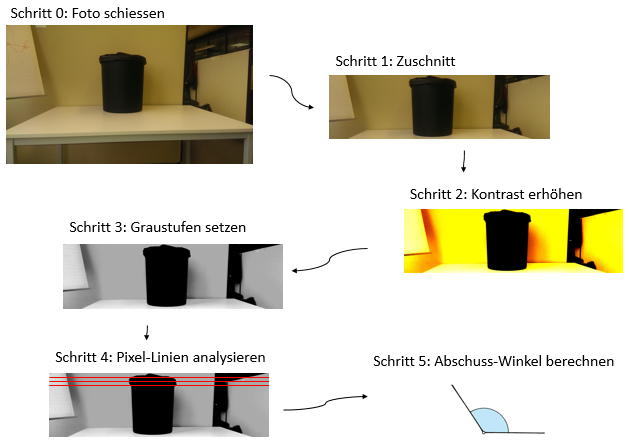
\includegraphics[width=0.7\linewidth]{../../fig/ablauf-ortung-des-korbes-algorithmus}
	\caption{Ablauf Erkennung des Korbes}
	\label{fig:ablauf-ortung-des-korbes-algorithmus}
\end{figure}

Sobald klar ist wo der Korb im Bild steht, werden die Pixel-Koordinaten zu Anzahl Schritte für den Schrittmotor konvertiert. Detaillierte Angaben zur Schnittstelle kann dem Abschnitt \ref{sec:schnittstelle-raspi-freedom} entnommen werden.
\\
\\
\textbf{Komponente Camera}
Mit dem Raspberry Pi wird eine Kamera über eine CSI-Schnittstelle\footnote{Camera Serial Interface} verbunden.  Die Kamera wird mit der Python-Bibliothek \texttt{picamera} angesteuert. Diese Bibliothek liefert das Bild als Python-Objekt zurück, welches danach direkt dem Algorithmus übergeben werden kann.
\\
\\
\textbf{Komponente Serial}
Hier ist eine Abstraktionsebene für den Webserver implementiert. Diese gilt als Vermittler zwischen Freedom-Board und Webserver. Das Freedom-Board wird über eine serielle Schnittstelle mit der Python-Bibliothek \texttt{pyserial} angesteuert.
\\
\\
\textbf{Komponente Freedom}
Das Freedom-Board, welches zuständig für die Motoren ist, ist über USB angeschlossen. Weitere Informationen dazu im Bereich der Elektrotechnik.
\\
\\
\textbf{Komponente Logger}
Diese Komponente ist zuständig für das Logging der Applikation. Log-Einträge werden entgegengenommen und in eine Datei gespeichert. Diese Einträge können entsprechend auch gelesen werden.
